\chapter{Construcción de Cable UTP y Plan de Pruebas de Certificación}

\section{Introducción y Objetivos}

La presente etapa constituye el componente de validación empírica y aseguramiento normativo del proyecto. Define:

\begin{enumerate}[leftmargin=*, label=\arabic*.]
    \item El protocolo metrológico de certificación de los 56 enlaces permanentes bajo la norma \textbf{ANSI/TIA-568-C.2}.
    \item El procedimiento exhaustivo de manufactura artesanal de la muestra física de cable UTP Cat~6 bajo la norma \textbf{T568B}.
    \item La taxonomía de fallas de cableado y el análisis del par dividido (\textit{Split Pair}).
    \item La guía de preparación para la evaluación individual aleatoria ante el docente.
    \item El formato formal de Hoja de Reporte de Certificación (\textit{Test Report Sheet}).
\end{enumerate}

\section{Plan de Pruebas y Certificación de Enlace Permanente}

\subsection{Enlace Permanente vs. Canal Completo}

La norma \textbf{ANSI/TIA-568.0-D} define dos configuraciones de medición con tolerancias distintas:

\begin{table}[H]
\caption{Diferenciación entre Enlace Permanente y Canal Completo}
\begin{tabularx}{\textwidth}{@{}lXX@{}}
\toprule
\textbf{Criterio} & \textbf{Enlace Permanente (\textit{Permanent Link})} & \textbf{Canal Completo (\textit{Channel})} \\
\midrule
Definición        & Infraestructura fija desde el terminal IDC del Patch Panel hasta el jack Keystone de pared & Enlace permanente más los dos latiguillos de ambos extremos \\
Longitud Máxima   & \textbf{90.0~m estrictos} & \textbf{100.0~m totales} ($90 + 10$~m de patch cords) \\
Exclusión         & El instrumento descuenta automáticamente sus adaptadores & Evalúa toda la ruta incluyendo conectores terminales \\
Uso en el Proyecto & \textbf{Modelo obligatorio para certificación y entrega de obra} (garantía 20 años) & Usado durante mantenimiento operativo \\
\bottomrule
\end{tabularx}
\label{tab:permanentlink}
\end{table}

\subsection{Parámetros Eléctricos y de RF Certificados (TIA-568-C.2)}

Cada uno de los 56 enlaces (50 UTP Cat~6 + 6 F/UTP Cat~6A) es sometido al barrido del certificador de campo Nivel~IIIe (\textit{Fluke DSX-5000 / DSX-8000}):

\begin{table}[H]
\caption{Parámetros de certificación y valores límite --- Cat~6 a 250~MHz}
\begin{tabularx}{\textwidth}{@{}lXcc@{}}
\toprule
\textbf{Parámetro} & \textbf{Descripción} & \textbf{Límite TIA Cat~6} & \textbf{Causa Típica de Falla} \\
\midrule
\textit{Wire Map}       & Continuidad pin a pin + pantalla (Cat~6A)              & 1:1 Continuo  & Error de pinout, corte al desforrar \\
\textit{Length (TDR)}   & Longitud medida por reflectometría (NVP $\approx 0.69c$)& $\leq 90.0$~m & Tirada excesiva de cable \\
\textit{IL} (Atenuación)& Pérdida de potencia de señal a 250~MHz                  & $\leq 31.1$~dB & Cable CCA o longitud excesiva \\
\textit{NEXT}           & Paradiafonía: inducción entre pares en extremo cercano  & $\geq 35.3$~dB & Destrenzado $>$ 13~mm al terminar \\
\textit{PS-NEXT}        & Suma de potencia de diafonía de 3 pares sobre el 4°     & $\geq 32.7$~dB & Precintos demasiado ajustados \\
\textit{Return Loss}    & Energía reflejada por variaciones de impedancia (100~$\Omega$) & $\geq 10.0$~dB & Quiebre por debajo del radio mínimo ($4\times$OD) \\
\textit{Delay / Skew}   & Tiempo de arribo y diferencia entre par más rápido/lento & Skew $\leq 45$~ns & Torsión despareja de fábrica \\
\bottomrule
\end{tabularx}
\label{tab:certificacion}
\end{table}

\subsubsection{Cálculo de Atenuación en el Enlace Más Lejano}

Para el enlace del Laboratorio Clínico (34.80~m), la atenuación estimada por la fórmula de la norma TIA es:

\begin{equation}
IL(250~\text{MHz}) \approx 32~\frac{\text{dB}}{100~\text{m}} \times \frac{34.80~\text{m}}{100~\text{m}} \approx 11.14~\text{dB}
\end{equation}

Esto genera un \textbf{margen favorable (\textit{headroom})} de casi 20~dB sobre el límite máximo de 31.1~dB.

\subsection{Diagnóstico de Fallas y el Par Dividido (\textit{Split Pair})}

\begin{table}[H]
\caption{Tipología de fallas en ensayos de cableado de par trenzado}
\begin{tabularx}{\textwidth}{@{}lXl@{}}
\toprule
\textbf{Tipo de Falla} & \textbf{Descripción} & \textbf{Detección} \\
\midrule
Circuito Abierto (\textit{Open})    & Conductor cortado o sin contacto en la cuchilla IDC            & Tester LED / Certificador \\
Cortocircuito (\textit{Short})      & Dos conductores en contacto eléctrico indeseado                & Tester LED / Certificador \\
Par Invertido (\textit{Reversed})   & Pines 1 y 2 intercambiados en un extremo                       & Tester LED / Certificador \\
Par Cruzado (\textit{Crossed})      & Un par entero en posiciones de otro                             & Tester LED / Certificador \\
\textbf{Par Dividido (\textit{Split Pair})} & Hilos de distintos pares mezclados idénticamente en ambos extremos & \textbf{Solo Certificador RF} \\
\bottomrule
\end{tabularx}
\label{tab:fallas}
\end{table}

El \textbf{par dividido} es la falla más peligrosa: un tester básico de LEDs muestra continuidad aparente 1:1 (falso aprobado), pero en la transmisión real la geometría de par trenzado balanceado se rompe, generando un \textbf{NEXT catastrófico de 10 a 15~dB} que impide la negociación Gigabit y provoca hasta el 80\% de pérdida de paquetes.

\begin{figure}[H]
\centering
\begin{tikzpicture}[scale=0.88, every node/.style={transform shape}]
    % Caso A: Cableado Normal (T568B)
    \node[font=\bfseries\small, text=mdpiBlue] at (3.5, 4.3) {A) Cableado Correcto T568B (Pares Balanceados)};
    \draw[fill=gray!10, rounded corners] (-0.3, -0.4) rectangle (7.3, 3.8);

    % Pines Extremo A y Extremo B
    \foreach \i in {1,...,8} {
        \node[circle, fill=black, text=white, inner sep=1.5pt, font=\tiny\bfseries] (A\i) at (0.5, 3.9 - 0.45*\i) {\i};
        \node[circle, fill=black, text=white, inner sep=1.5pt, font=\tiny\bfseries] (B\i) at (6.5, 3.9 - 0.45*\i) {\i};
    }
    % Líneas de pares
    \draw[line width=1.5pt, orange] (A1) -- (B1);
    \draw[line width=1.5pt, orange!70!black] (A2) -- (B2);
    \draw[line width=1.5pt, green!60!black] (A3) -- (B3);
    \draw[line width=1.5pt, blue] (A4) -- (B4);
    \draw[line width=1.5pt, blue!70!black] (A5) -- (B5);
    \draw[line width=1.5pt, green!60!black] (A6) -- (B6);
    \draw[line width=1.5pt, brown] (A7) -- (B7);
    \draw[line width=1.5pt, brown!70!black] (A8) -- (B8);

    \node[right, font=\tiny, text=green!60!black] at (2.2, 0.3) {NEXT $>$ 35~dB: \textbf{APROBADO}};

    % Caso B: Par Dividido (Split Pair)
    \begin{scope}[xshift=8.5cm]
        \node[font=\bfseries\small, text=red!80!black] at (3.5, 4.3) {B) Par Dividido / Split Pair (Falso Aprobado en LED)};
        \draw[fill=red!5, draw=red!40, rounded corners] (-0.3, -0.4) rectangle (7.3, 3.8);

        \foreach \i in {1,...,8} {
            \node[circle, fill=black, text=white, inner sep=1.5pt, font=\tiny\bfseries] (SA\i) at (0.5, 3.9 - 0.45*\i) {\i};
            \node[circle, fill=black, text=white, inner sep=1.5pt, font=\tiny\bfseries] (SB\i) at (6.5, 3.9 - 0.45*\i) {\i};
        }
        % Continuidad DC es 1:1
        \draw[line width=1.5pt, orange] (SA1) -- (SB1);
        \draw[line width=1.5pt, orange!70!black] (SA2) -- (SB2);
        % Error: Hilo de Par 3 mezclado en vaina con hilo de Par 1
        \draw[line width=1.5pt, red, dashed] (SA3) -- (SB3);
        \draw[line width=1.5pt, red, dashed] (SA4) -- (SB4);
        \draw[line width=1.5pt, blue!70!black] (SA5) -- (SB5);
        \draw[line width=1.5pt, green!60!black] (SA6) -- (SB6);
        \draw[line width=1.5pt, brown] (SA7) -- (SB7);
        \draw[line width=1.5pt, brown!70!black] (SA8) -- (SB8);

        \draw[{Latex[length=2mm]}-{Latex[length=2mm]}, red, line width=1pt] (3.5, 2.5) -- (3.5, 2.1);
        \node[font=\tiny\bfseries, text=red] at (3.5, 1.8) {Fuerte acoplamiento RF};
        \node[right, font=\tiny, text=red] at (1.8, 0.3) {NEXT $< 15$~dB: \textbf{FALLA CRÍTICA}};
    \end{scope}
\end{tikzpicture}
\caption{Comparativa entre canal balanceado T568B y defecto electromagnético de Par Dividido (\textit{Split Pair})}
\label{fig:splitpair}
\end{figure}

\begin{figure}[H]
\centering
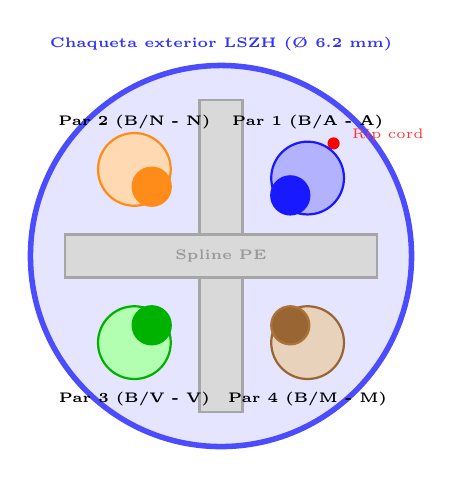
\begin{tikzpicture}[scale=1.1]
    % Chaqueta exterior LSZH
    \draw[fill=blue!10, draw=blue!70, line width=2pt] (0,0) circle (2.2cm);
    \node[font=\tiny\bfseries, text=blue!80] at (0, 2.45) {Chaqueta exterior LSZH (Ø 6.2 mm)};

    % Cruceta plástica separadora central (Spline)
    \draw[fill=gray!30, draw=gray!70, line width=1pt] (-0.25, -1.8) rectangle (0.25, 1.8);
    \draw[fill=gray!30, draw=gray!70, line width=1pt] (-1.8, -0.25) rectangle (1.8, 0.25);
    \node[font=\tiny\bfseries, text=gray!80] at (0, 0) {Spline PE};

    % Hilo de rasgado (Rip cord)
    \fill[red] (1.3, 1.3) circle (2pt);
    \node[font=\tiny, text=red!80, anchor=west] at (1.4, 1.4) {Rip cord};

    % Par 2 (Naranja) - Superior Izquierda
    \draw[fill=orange!30, draw=orange!90, line width=0.8pt] (-1.0, 1.0) circle (0.42cm);
    \draw[fill=orange!90, draw=orange!90, line width=0.8pt] (-0.8, 0.8) circle (0.22cm);
    \node[font=\tiny\bfseries] at (-1.0, 1.55) {Par 2 (B/N - N)};

    % Par 1 (Azul) - Superior Derecha
    \draw[fill=blue!30, draw=blue!90, line width=0.8pt] (1.0, 0.9) circle (0.42cm);
    \draw[fill=blue!90, draw=blue!90, line width=0.8pt] (0.8, 0.7) circle (0.22cm);
    \node[font=\tiny\bfseries] at (1.0, 1.55) {Par 1 (B/A - A)};

    % Par 3 (Verde) - Inferior Izquierda
    \draw[fill=green!30, draw=green!70!black, line width=0.8pt] (-1.0, -1.0) circle (0.42cm);
    \draw[fill=green!70!black, draw=green!70!black, line width=0.8pt] (-0.8, -0.8) circle (0.22cm);
    \node[font=\tiny\bfseries] at (-1.0, -1.65) {Par 3 (B/V - V)};

    % Par 4 (Marrón) - Inferior Derecha
    \draw[fill=brown!35, draw=brown!80!black, line width=0.8pt] (1.0, -1.0) circle (0.42cm);
    \draw[fill=brown!80!black, draw=brown!90!black, line width=0.8pt] (0.8, -0.8) circle (0.22cm);
    \node[font=\tiny\bfseries] at (1.0, -1.65) {Par 4 (B/M - M)};
\end{tikzpicture}
\caption{Corte transversal y anatomía física del cable UTP Categoría 6 monofilamento 23~AWG}
\label{fig:cablecat6}
\end{figure}

\section{Guía de Fabricación de la Muestra Física UTP (T568B)}

\subsection{Materiales Necesarios}

\begin{itemize}[leftmargin=*]
    \item 2.0~m de cable UTP Cat~6 monofilamento 23~AWG, 100\% cobre, forro LSZH.
    \item 2 conectores machos RJ-45 (8P8C) Cat~6 con contactos dorados de 50~$\mu$in y guía escalonada.
    \item 2 capuchones de goma termoplástica protectores de lengüeta.
    \item Herramienta pelacables rotativa, ponchadora de trinquete y tester de continuidad.
\end{itemize}

\subsection{Procedimiento Paso a Paso}

\begin{enumerate}[leftmargin=*, label=\textbf{Paso \arabic*.}]
    \item \textbf{Capuchones:} Deslizar un capuchón en cada extremo del cable (sentido invertido) \textit{antes} de desforrar.
    
    \item \textbf{Desforrado:} Retirar exactamente \textbf{30~mm} de chaqueta exterior con la herramienta pelacables calibrada, sin mellar el aislamiento interno de los 8 conductores.
    
    \item \textbf{Retiro de elementos pasivos:} Cortar al ras con alicate diagonal el hilo de rasgado (\textit{rip cord}) y el separador cruciforme (\textit{spline}).
    
    \item \textbf{Ordenamiento T568B:} Destrenzar los pares \textbf{no más de 13~mm} desde la chaqueta. Ordenar de izquierda a derecha (pestaña del conector hacia abajo):
    \begin{equation*}
        \underbrace{\text{B/Naranja}}_{\text{Pin 1}} - \underbrace{\text{Naranja}}_{\text{Pin 2}} - \underbrace{\text{B/Verde}}_{\text{Pin 3}} - \underbrace{\text{Azul}}_{\text{Pin 4}} - \underbrace{\text{B/Azul}}_{\text{Pin 5}} - \underbrace{\text{Verde}}_{\text{Pin 6}} - \underbrace{\text{B/Marrón}}_{\text{Pin 7}} - \underbrace{\text{Marrón}}_{\text{Pin 8}}
    \end{equation*}
    
    \item \textbf{Corte a 90°:} Recortar con corte perpendicular dejando \textbf{13 a 14~mm} de conductores expuestos desde la chaqueta.
    
    \item \textbf{Inserción:} Deslizar en el conector RJ-45 hasta que los 8 conductores toquen visualmente el frente transparente. \textbf{Criterio crítico:} la chaqueta debe ingresar al menos \textbf{6~mm} dentro del cuerpo del conector para ser prensada por la cuña de retención mecánica.
    
    \item \textbf{Crimpado:} Colocar en el puerto 8P de la ponchadora de trinquete y presionar hasta liberar el seguro. Las 8 cuchillas doradas perforan el aislamiento por desplazamiento (\textit{IDC}).
    
    \item \textbf{Verificación:} Conectar a tester de continuidad (Master + Remote). Los LEDs del 1 al 8 deben encenderse en \textbf{secuencia sincrónica y verde}, confirmando la ausencia de cortes, pares cruzados o falsos contactos.
\end{enumerate}

\section{Guía para la Evaluación Individual Aleatoria}

\subsection{Preguntas Típicas de Sustentación y Respuestas Esperadas}

\subsubsection{¿Por qué se eligió T568B frente a T568A?}

La norma T568B es el estándar de facto en Perú y Latinoamérica. Únicamente cambian de posición los \textbf{Pares 2 (Naranja) y 3 (Verde)} entre ambos esquemas. En T568A, los pines 1--2 son Blanco/Verde y Verde; en T568B son Blanco/Naranja y Naranja. Los pares 1 (Azul, pines 4--5) y 4 (Marrón, pines 7--8) son idénticos en ambas normas.

\subsubsection{¿Por qué la norma prohíbe destrenzar más de 13~mm?}

El trenzado de los pares de cobre es el principio físico que cancela el ruido electromagnético externo y la paradiafonía (NEXT) entre pares adyacentes mediante inducción mutua balanceada. Si se destrenza más de 13~mm, los conductores se comportan como líneas paralelas sin blindaje, provocando que el NEXT decaiga estrepitosamente e impidiendo la certificación a 250~MHz y la negociación Gigabit.

\subsubsection{Si los LEDs 1 y 2 no encienden en el tester, ¿qué falla indica?}

Indica un \textbf{Circuito Abierto (\textit{Open})} en el Par 2 (Naranja/Blanco-Naranja). Causas: (1) Los hilos no llegaron al fondo del conector antes del crimpado y las cuchillas no perforaron el aislamiento; (2) Los conductores fueron cortados accidentalmente al desforrar la chaqueta con el pelacables.

\subsubsection{¿Para qué servía el cable cruzado y por qué hoy se usa solo cable directo?}

El cable cruzado (T568A en un extremo, T568B en el otro) se usaba en redes 10BASE-T y 100BASE-TX para interconectar dispositivos del mismo tipo (PC a PC, switch a switch), cruzando los pines Tx y Rx. Actualmente todos los equipos implementan \textbf{Auto-MDIX (IEEE~802.3ab)}, que detecta y conmuta automáticamente por software los pares de transmisión y recepción, haciendo que toda la infraestructura opere exclusivamente con cables directos T568B.

\section{Ficha Técnica de Reporte de Certificación}

\begin{table}[H]
\caption{Reporte de certificación de enlace permanente --- Ejemplo (R1-PP1-P15 / C01-D1)}
\begin{tabularx}{\textwidth}{@{}lXl@{}}
\toprule
\textbf{Parámetro} & \textbf{Valor Medido} & \textbf{Estado} \\
\midrule
Identificador TIA-606 & R1-PP1-P15 / C01-D1 (Consultorio 01 --- PC Médica) & --- \\
Tipo de cable         & UTP Cat~6 LSZH 23~AWG sólido                       & --- \\
Longitud medida       & 13.20~m ($\leq 90.0$~m)                             & \textbf{PASA} \\
Wire Map              & 1:1 directo (8 pines)                               & \textbf{PASA} \\
Resistencia DC        & 2.85~$\Omega$ ($\leq 18.0$~$\Omega$)                & \textbf{PASA} \\
IL a 250~MHz          & 4.12~dB ($\leq 31.10$~dB)                          & \textbf{PASA} \\
NEXT a 250~MHz        & 54.80~dB ($\geq 35.30$~dB)                         & \textbf{PASA} \\
PS-NEXT               & 51.20~dB ($\geq 32.70$~dB)                         & \textbf{PASA} \\
Return Loss           & 21.40~dB ($\geq 10.00$~dB)                         & \textbf{PASA} \\
Delay                 & 68.40~ns ($\leq 498.00$~ns)                        & \textbf{PASA} \\
Delay Skew            & 9.80~ns ($\leq 45.00$~ns)                          & \textbf{PASA} \\
\midrule
\multicolumn{2}{l}{\textbf{Dictamen Final}} & \textbf{APROBADO --- ANSI/TIA-568-C.2} \\
\bottomrule
\end{tabularx}
\label{tab:test-report}
\end{table}
